\documentclass{article}
\usepackage[utf8]{inputenc}
\usepackage[letterpaper, margin=0.80in]{geometry}
\usepackage{graphicx}
\graphicspath{ {./images/} }
\usepackage{amsmath}
\usepackage{graphicx}
\graphicspath{ {images/} }
\usepackage{amssymb}
\usepackage{verbatim}
\usepackage{xparse}
\newcommand*\Eval[3]{\left.#1\right\rvert_{#2}^{#3}}
\usepackage{pgfplots}
\usepackage{listings}
\pgfplotsset{width=10cm,compat=1.9}
\usepgfplotslibrary{external}
\tikzexternalize
\documentclass{book}
\usepackage{hyperref}
\hypersetup{
    colorlinks=true,
    linkcolor=cyan,
    filecolor=cyan,
    urlcolor=cyan,
    pdftitle={Overleaf Example},
    pdfpagemode=FullScreen,
    }

\title{Optimization of Path-Time of a Formula 1 Vehicle on a Race Track}
\author{Vedansh Goenka, Jackson Goenawan, and Robert Griswold}
\date{May 12th, 2022}

\begin{document}
\maketitle
\section{Introduction}
\subsection{Formula 1}

Formula 1 (F1) is the highest level of open-wheel racing. It includes the world's most skilled drivers and the manufacturers develop unique, specialized cars for this specific purpose, as opposed to other classes of racing where the cars are based off of street cars. Formula 1 has developed into a form of a professional sport. The season is around 8-9 months long and consists of roughly 22 races, namely “grands prix". There are 10 manufacturing teams with 2 drivers competing within each team, totaling 20 cars in a race. Grands prix consist of three parts: free-practice, qualifying, and the consequent main race. Qualifying rounds determine the starting position of the cars for the race itself, and it is this qualifying session that we are going to be focusing on. Qualifying is where each driver goes out on the track, on their own, with no other cars on the track to set the fastest lap-time they possibly can without any interference. The slowest 5 are eliminated, and the process is repeated until the order is determined. We are focusing on this qualifying lap because there are no other drivers, or obstacles, to work around. It is just the car and the track.

\subsection{Racing Line}

A contentious area of F1 races, and all racing, is the optimal path through a corner, and thus, through an entire track to minimize total lap-time. This theoretical path is what we will refer to as the racing line. In the racing community, it is often accepted that the racing line through an isolated corner will be the path with the largest overall radius, allowing for maximum speed throughout the corner. However, the geometry of the corner itself and the context of the track around it alter this theoretical path. Formula 1 tracks are compiled of three distinct components: corners, straights, and chicanes. Corners are curved portions of the track in a single direction, straights are straight portions of the track, and chicanes are two corners lined up end to end in opposite directions. The objective of this project is to determine the racing line through a specific corner.

\section{Governing Equation}
\subsection{Derivation}

\centering From Newton's Second Law:

\begin{equation}
    \sum F=m*a
\end{equation}

\centering Creating a vector sum for the net forces in the X and Y directions and setting them equal to the force of friction on the tires:

\begin{equation}
    \mu_F(mg+\mu_Av_x) = \sqrt{(ma_x - \mu_Dv_x^2)^2 + (\frac{mv_x^2}{r})^2}
\end{equation}

\begin{equation}
    \mu_Fmg+\mu_F\mu_Av^2 = \frac{mv^2}{r}
\end{equation}

Solve for v,

\begin{equation}
    v_{max}=\sqrt{\frac{\mu_Fmg}{\frac{m}{r}-\mu_F\mu_A}}
\end{equation}

\begin{equation}
    f(\Delta t) = \alpha (\Delta t)^2 e^{-\beta(\Delta t)} + (1-e^{-\beta\Delta t})(\gamma (\Delta t)^2 + \delta)-\Delta t
\end{equation}

\begin{equation}
    f'(\Delta t) = e^{-\beta(\Delta t)}((2\gamma - 1)e^{\beta (\Delta t)} + (\gamma - \alpha)(\beta (\Delta t) -2)(\Delta t) + B\delta)
\end{equation}

\begin{equation}
    \text{Let } \alpha = \frac{v_L}{r\Delta \theta} \text{, } \beta = \frac{\mu_F\mu_A\mu_Dr}{m^2} \text{; } \gamma = -\frac{mg}{\mu_Ar(\Delta \theta)} \text{; } \delta = \frac{mr(\Delta\theta)\mu_D + m^2}{\mu_F\mu_A\mu_Dr}
\end{equation}

\begin{equation}
    \Delta t_{n+1} = \Delta t + \frac{f(\Delta t)}{f'(\Delta t)}
\end{equation}


\subsubsection{Variables}
\begin{center}
\begin{tabular}{ |c|c| }
 \hline
 \mu_A = \frac{1}{2}\rho S C_L & rolled coefficient of aerodynamic negative lift\\ [.2ex]
 \hline
 \mu_D = \frac{1}{2}\rho C_DA & rolled coefficient of aerodynamic drag\\ [.2ex]
 \hline
 \mu_F & coefficient of friction \\[.2ex]
 \hline
 r & radius of discretized track location \\ [.2ex]
 \hline
 \Delta \theta & angular displacement through path \\[.2ex]
 \hline
 m & mass of vehicle \\[.2ex]
 \hline
 g & gravitation acceleration constant \\[.2ex]
 \hline
\end{tabular}
\end{center}


\subsubsection{values}
\begin{center}
\begin{tabular}{ |c|c| }
 \hline
 \mu_A & 0.150698949^\hyperref[sec:bib]{7}\\
 \hline
 m & 905^\hyperref[sec:bib]{3} \\
 \hline
 \mu_D & 0.128311639^\hyperref[sec:bib]{7} \\
 \hline
 \mu_F & 1.7^\hyperref[sec:bib]{8} \\
 \hline
\end{tabular}
\end{center}

\raggedright
\subsection{Assumptions}

\begin{enumerate}

\item There is no camber. Camber is simply how banked a corner is. For the purposes of this project, we are assuming that the track is completely flat.
\item It is a static car. We are concentrating all the forces on the car to the center of mass. This allows us to compile everything in one equation and eliminate any torsional forces across the car and unequal forces across the tires as a result of weight transfer and to assume that drag, lift, friction, and gravity all act at the same place, the center of mass. In reality, these forces would reduce the efficiency of the car through the turn.

\item The conditions of the car are constant, meaning that the coefficient of friction between the tires and the track is constant, the rolled coefficient of aerodynamic drag is constant, and the rolled coefficient of aerodynamic negative lift is constant. In reality, the tires would both wear down and heat up, changing the coefficient of friction. Additionally, the Drag Reduction Systems on Formula 1 vehicles makes the coefficient of drag and the coefficient of aerodynamic lift variable.

\item The track conditions are ideal and constant. In reality, certain areas of the track have different coefficients of friction between the track and the tires due to rubber on the track, water, and temperature.

\end{enumerate}

\section{Implementation}

\subsection{Discretization of the Track}
To utilize our governing equation, we discretized the corner into many small arcs. From there, we can determine the path with the shortest change in time to either the next cell on the current radius, or to the adjacent cell on either side. Running this repeatedly, we generate the fastest path through a single corner. For our benchmarking, we will be using the first 2 corners from the Jeddah Grand Prix.
\break \break

Overlaying a grid onto an overhead image of the corner, we can use the rear width of the car, which is a specified length according to the FIA Formula 1 regulation manual, to obtain the dimensions of the track using Fusion 360:
\begin{center} 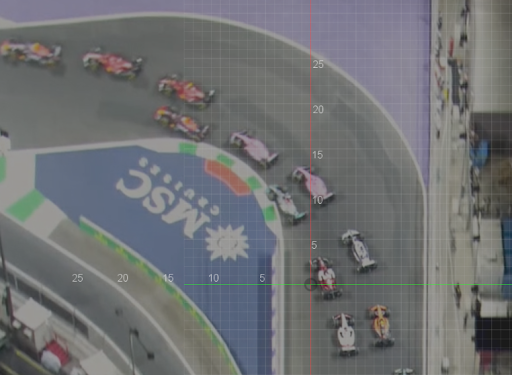
\includegraphics[scale=.75]{unnamed-7} \end{center}
\break
\break

Next, we overlay arcs, lines, and splines to define the track. We then split up the track based on the discretization parameters: \break
\begin{center} 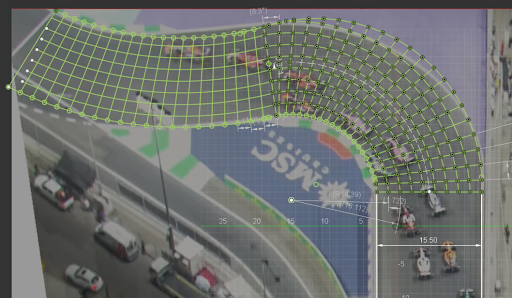
\includegraphics[scale=.75]{unnamed-6} \end{center}
\break
\break

Once the track is split up, we extract the radius, the change in theta, and the change in radius as you move in and out of the track \break
\begin{center} 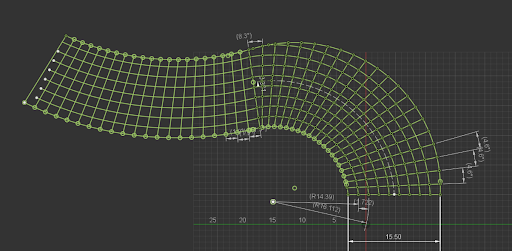
\includegraphics[scale=.75]{unnamed-5} \end{center}


\subsection{Creating the Matrix}
Using the information extracted from the discretization of the track, we create a matrix for this corner. For this instance, it is 9 by 40, representing the 9 possible positions across the track laterally and the 40 steps through the corner. Each cell in the matrix, represented below, has the radius and delta theta for that individual segment of track.
\break

\centering \begin{bmatrix}
(r,\theta)_{0,0}, & (r,\theta)_{0,1}, & \ldots & (r,\theta)_{0,8}\\
(r,\theta)_{1,0}, & (r,\theta)_{1,1}, & \ldots & (r,\theta)_{1,8}\\
\vdots & \vdots & & \vdots \\
(r,\theta)_{39,0}, & (r,\theta)_{39,1}, & \ldots & (r,\theta)_{39,8}
\end{bmatrix}

\raggedright
\subsection{Generating the Path}
To generate the fastest path, we take the current position of the car on the track, and then calculate the three cells it can travel to. The possible positions are in the next row, in the same column as the previous position, or the two cells adjacent to it. This generates three different paths, each with a different radius. Calculating the change in time required to travel to each of the three positions, we choose the path with the smallest change in time.
\break \break
Running this 40 times, we generate a full path through the corner. Our resulting path starts from the outside and cuts into the inside of the track before cutting back to the outside of the track.
\begin{center} 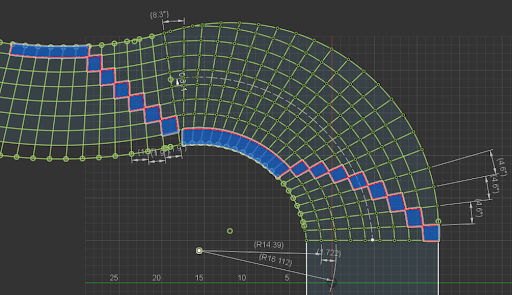
\includegraphics[scale=.75]{unnamed-2} \end{center}

\subsection{Benchmarking}
When overlaying this onto the actual path of the Formula 1 cars, we find that the general path aligns with the vehicles' paths. The photo imaged below shows some cars differing from the optimal path, as the photograph was not from qualifying. Instead, the other cars on the track added complexity and acted as obstacles, altering the optimal path of the vehicle.
\begin{center} 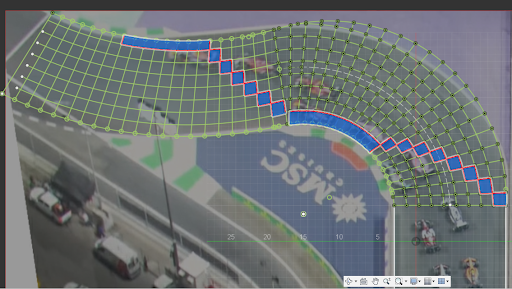
\includegraphics[scale=.75]{unnamed} \end{center}
\break \break
In this theoretical model with the ideal car and track conditions, we obtained a time of 2.75 seconds to travel through the corner. Lewis Hamilton, a Mercedes Formula 1 driver, took \href{https://www.youtube.com/watch?v=ugJ-rYS-9JU}{3.2 seconds} to travel through the corner in his qualifying lap. The difference between the theoretical and actual time is most likely due to the car and the track not being ideal. In our model, the track conditions are perfect and constant, while the car lacks any torsional forces and imbalances.

\subsection{Improvements}
There is a lot that we can continue to do and improve with this project. Firstly, we can vary the track conditions at each discrete point, allowing us to simulate the effect of rubber being embedded into the track, increasing the coefficient of friction over a specific area, or to simulate rain on areas of the track. Secondly, we can discretize a full track rather than a specific corner to get the optimal path for the entire lap. Additionally, we can "look ahead" using the Runge-Kutta 4 method to effectively test every possible path throughout the track and obtain a more optimal line when considering more than just a single corner. Finally, we can remove some of the assumptions we made that most likely had a large impact on the results.





\newpage
\begin{thebibliography}{9}
\label{sec:bib}

\bibitem{Corner Analysis}
``Corner Analysis.'' \textit{Amazon Web Services, Inc.} \url{aws.amazon.com/f1/corner-analysis/}

\bibitem{Poop in car}
\textit{Do F1 Drivers Poop & Pee in Their Cars?} 10 Feb 2022, \url{www.essentiallysports.com/stories/f1-news-do-f1-drivers-poop-pee-in-their-cars.} Accessed 17 May 2022.

\bibitem{hamilton}
Formula1. ``Lewis Hamilton's Pole Lap | 2021 Saudi Arabian Grand Prix | Pirelli.'' \textit{YouTube,} YouTube, 4 Dec. 2021, \url{https://www.youtube.com/watch?v=ugJ-rYS-9JU.}

\bibitem{vedansh}
Goenka, Vedansh. ``Calc3FinalProject.'' \textit{Github,} \url{https://github.com/VedanshGoenka/Calc3FinalProject.}

\bibitem{Horton}
Horton, Phillip. ``Why F1 Cars in 2022 Will Be Heaviest of the Hybrid Era.''\textit{Autoweek,} 7 Jan. 2022, \url{www.autoweek.com/racing/formula-1/a38695541/why-f1-cars-2022-heaviest-hybrid-era.}

\bibitem{Jeddah}
``Jeddah Corniche Circuit.'' \textit{Formula 1 Wiki,} \url{1.fandom.com/wiki/Jeddah_Corniche_Circuit.} Accessed 17 May 2022.

\bibitem{Jiang}
Jiang, Kun, et al. ``Real-Time Estimation and Prediction of Tire Forces Using Digital Map for Driving Risk Assessment.'' \textit{Transportation Research Part C: Emerging Technologies,} vol. 107, Oct. 2019, pp. 463–489, 10.1016/j.trc.2019.08.016.

\bibitem{Ramanata}
Ramanata, Peeroon Pete. ``Optimal Vehicle Path Generator Using Optimization Methods.'' \textit{Vtechworks.lib.vt.edu,} 15 Apr. 1998, \url{vtechworks.lib.vt.edu/handle/10919/36615} Accessed 17 May 2022.

\bibitem{Jordan}
Smith, Jordan. \textit{Formula One Car Downforce Analysis.}

\bibitem{HPwizard}
``Tire Friction and Rolling Coefficients.'' \textit{Hpwizard.com,} 2010, \url{hpwizard.com/tire-friction-coefficient.html.}

\bibitem{Quora}
``What Is the "Racing Line" in Auto Racing?'' \textit{Quora,} \url{www.quora.com/What-is-the-racing-line-in-auto-racing/answer/Sean-McKiernan?ch=10&oid=135887534&share=8d89d393&srid=6wSUF&target_type=answer.} Accessed 17 May 2022.

\end{thebibliography}

\end{document}